\chapter{Results and Discussion}

\section{Sequences and Static Structures}
\begin{figure}[h!]
	\label{MSA + RMSDs}
	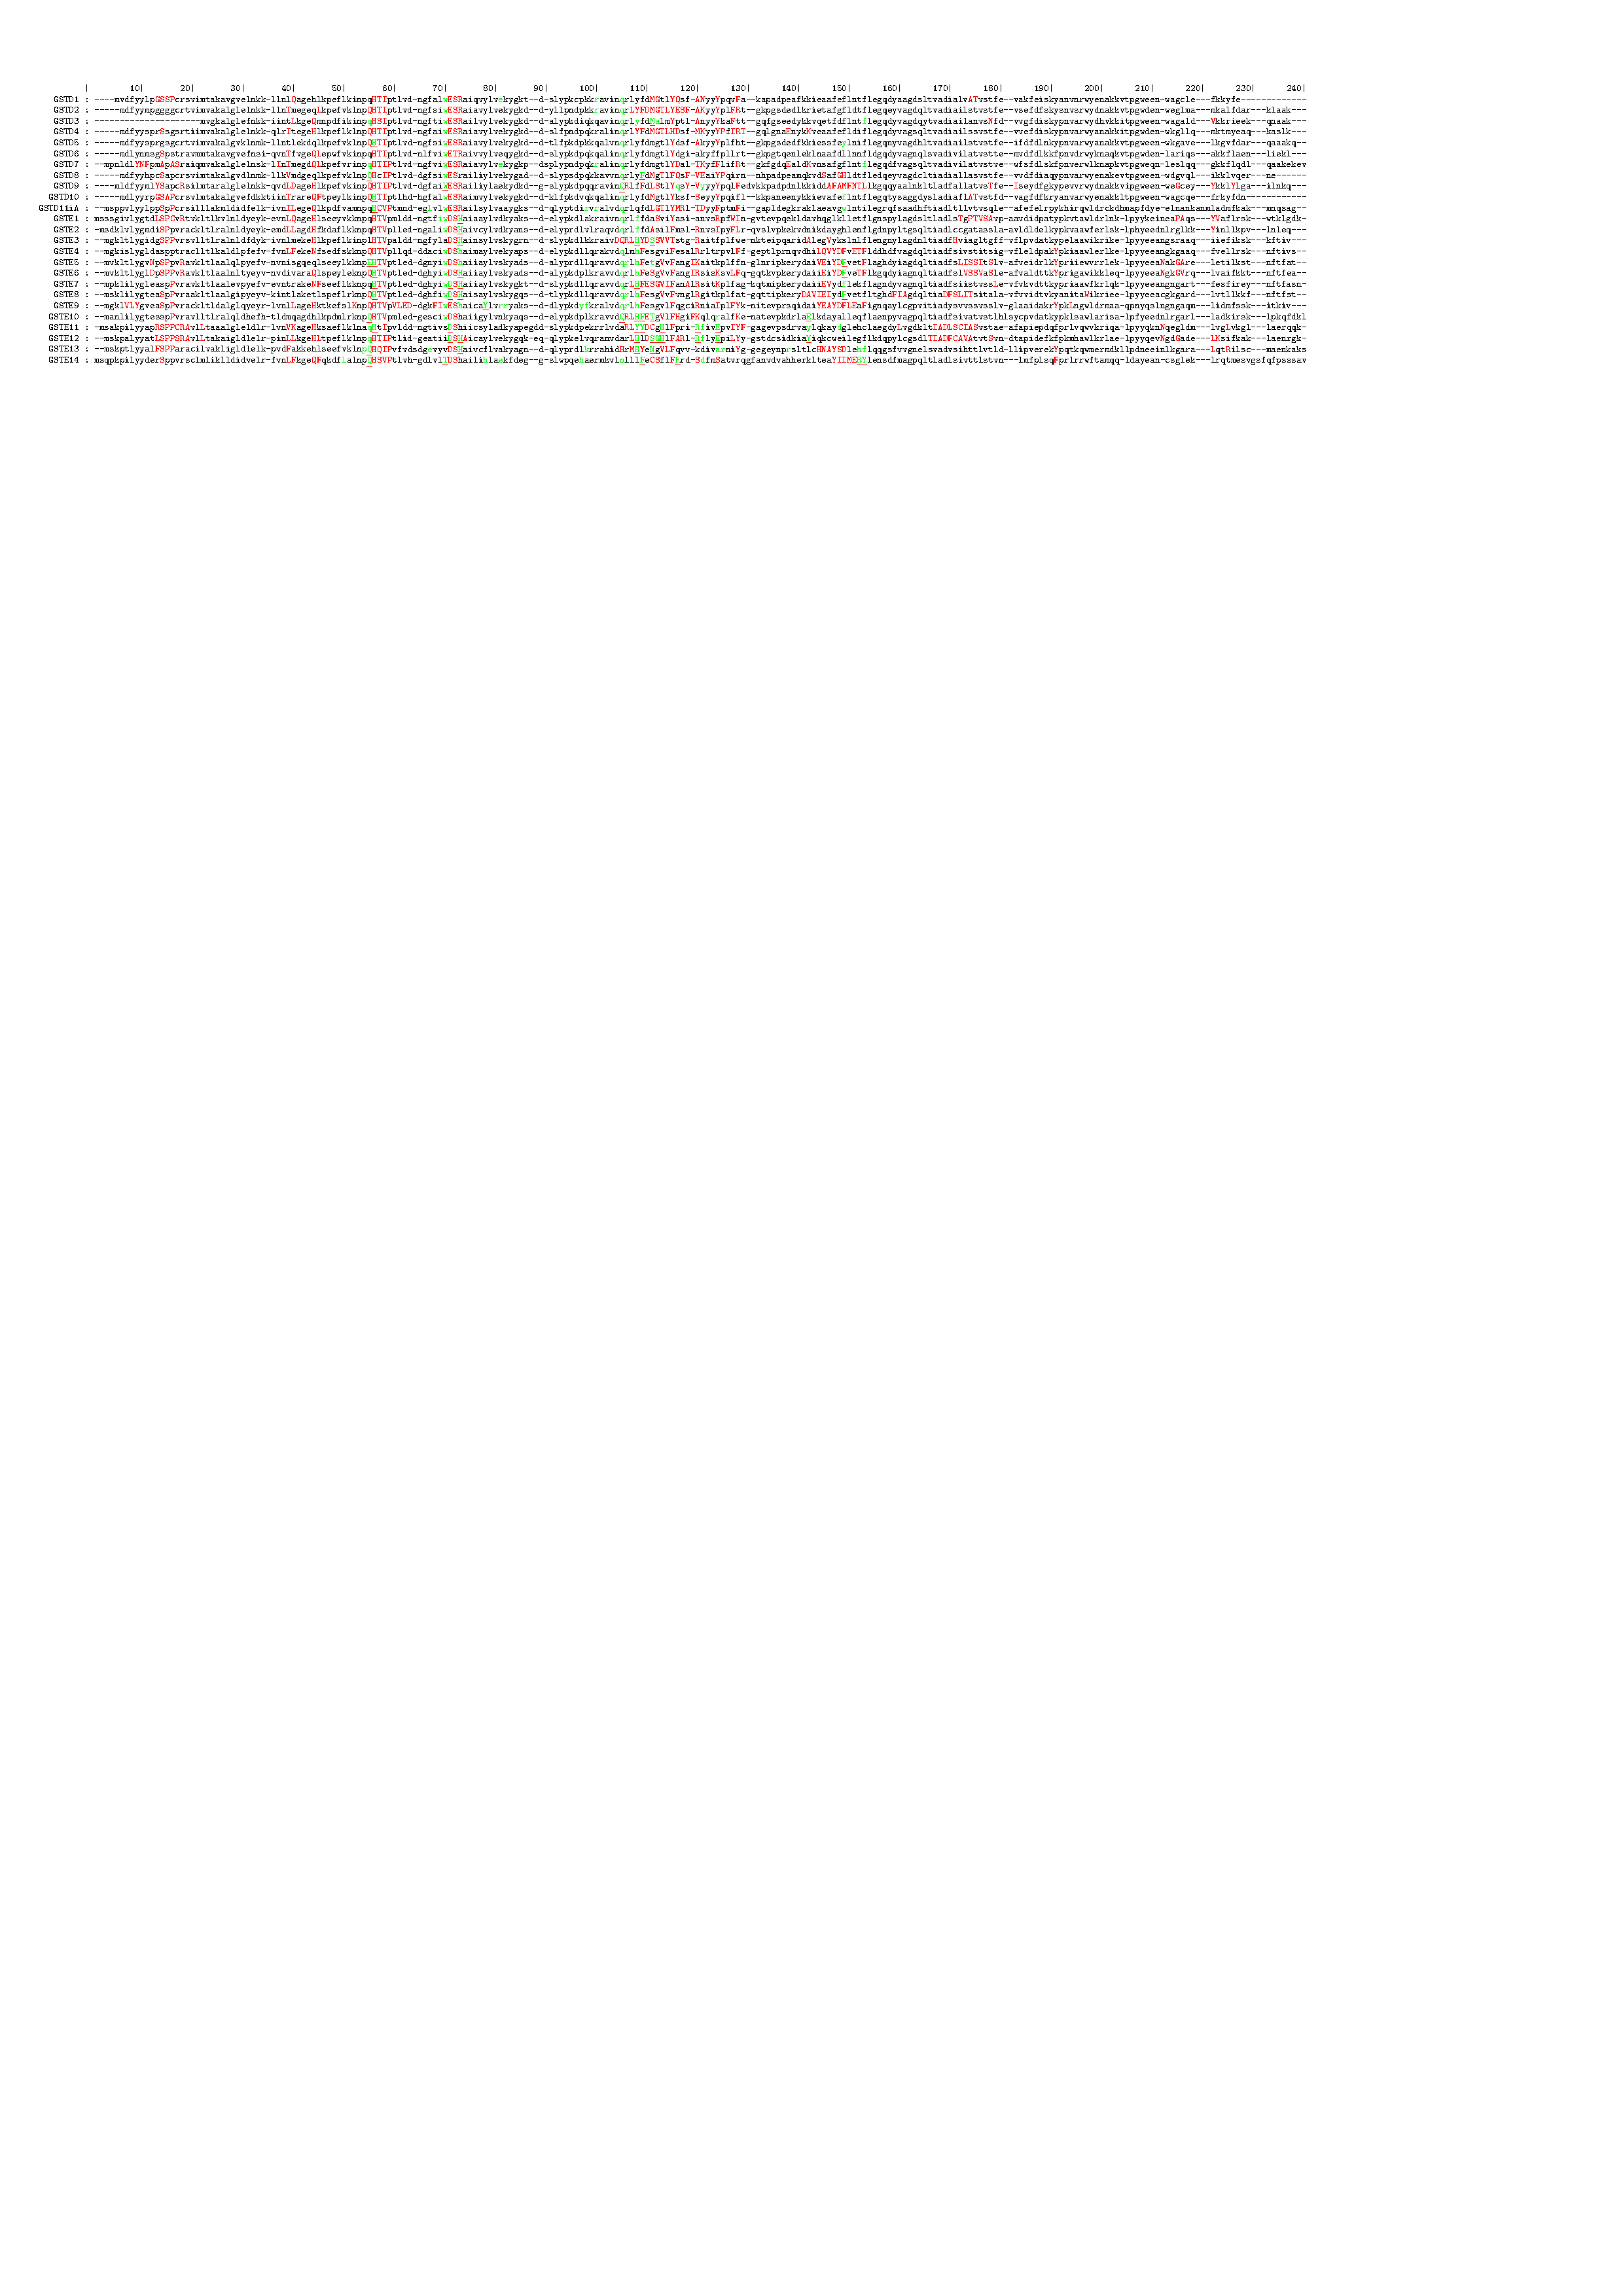
\includegraphics[width = .99\textwidth]{figures/MSA_matrix.pdf}\\[.5cm]
	\begin{minipage}{.32\linewidth}
		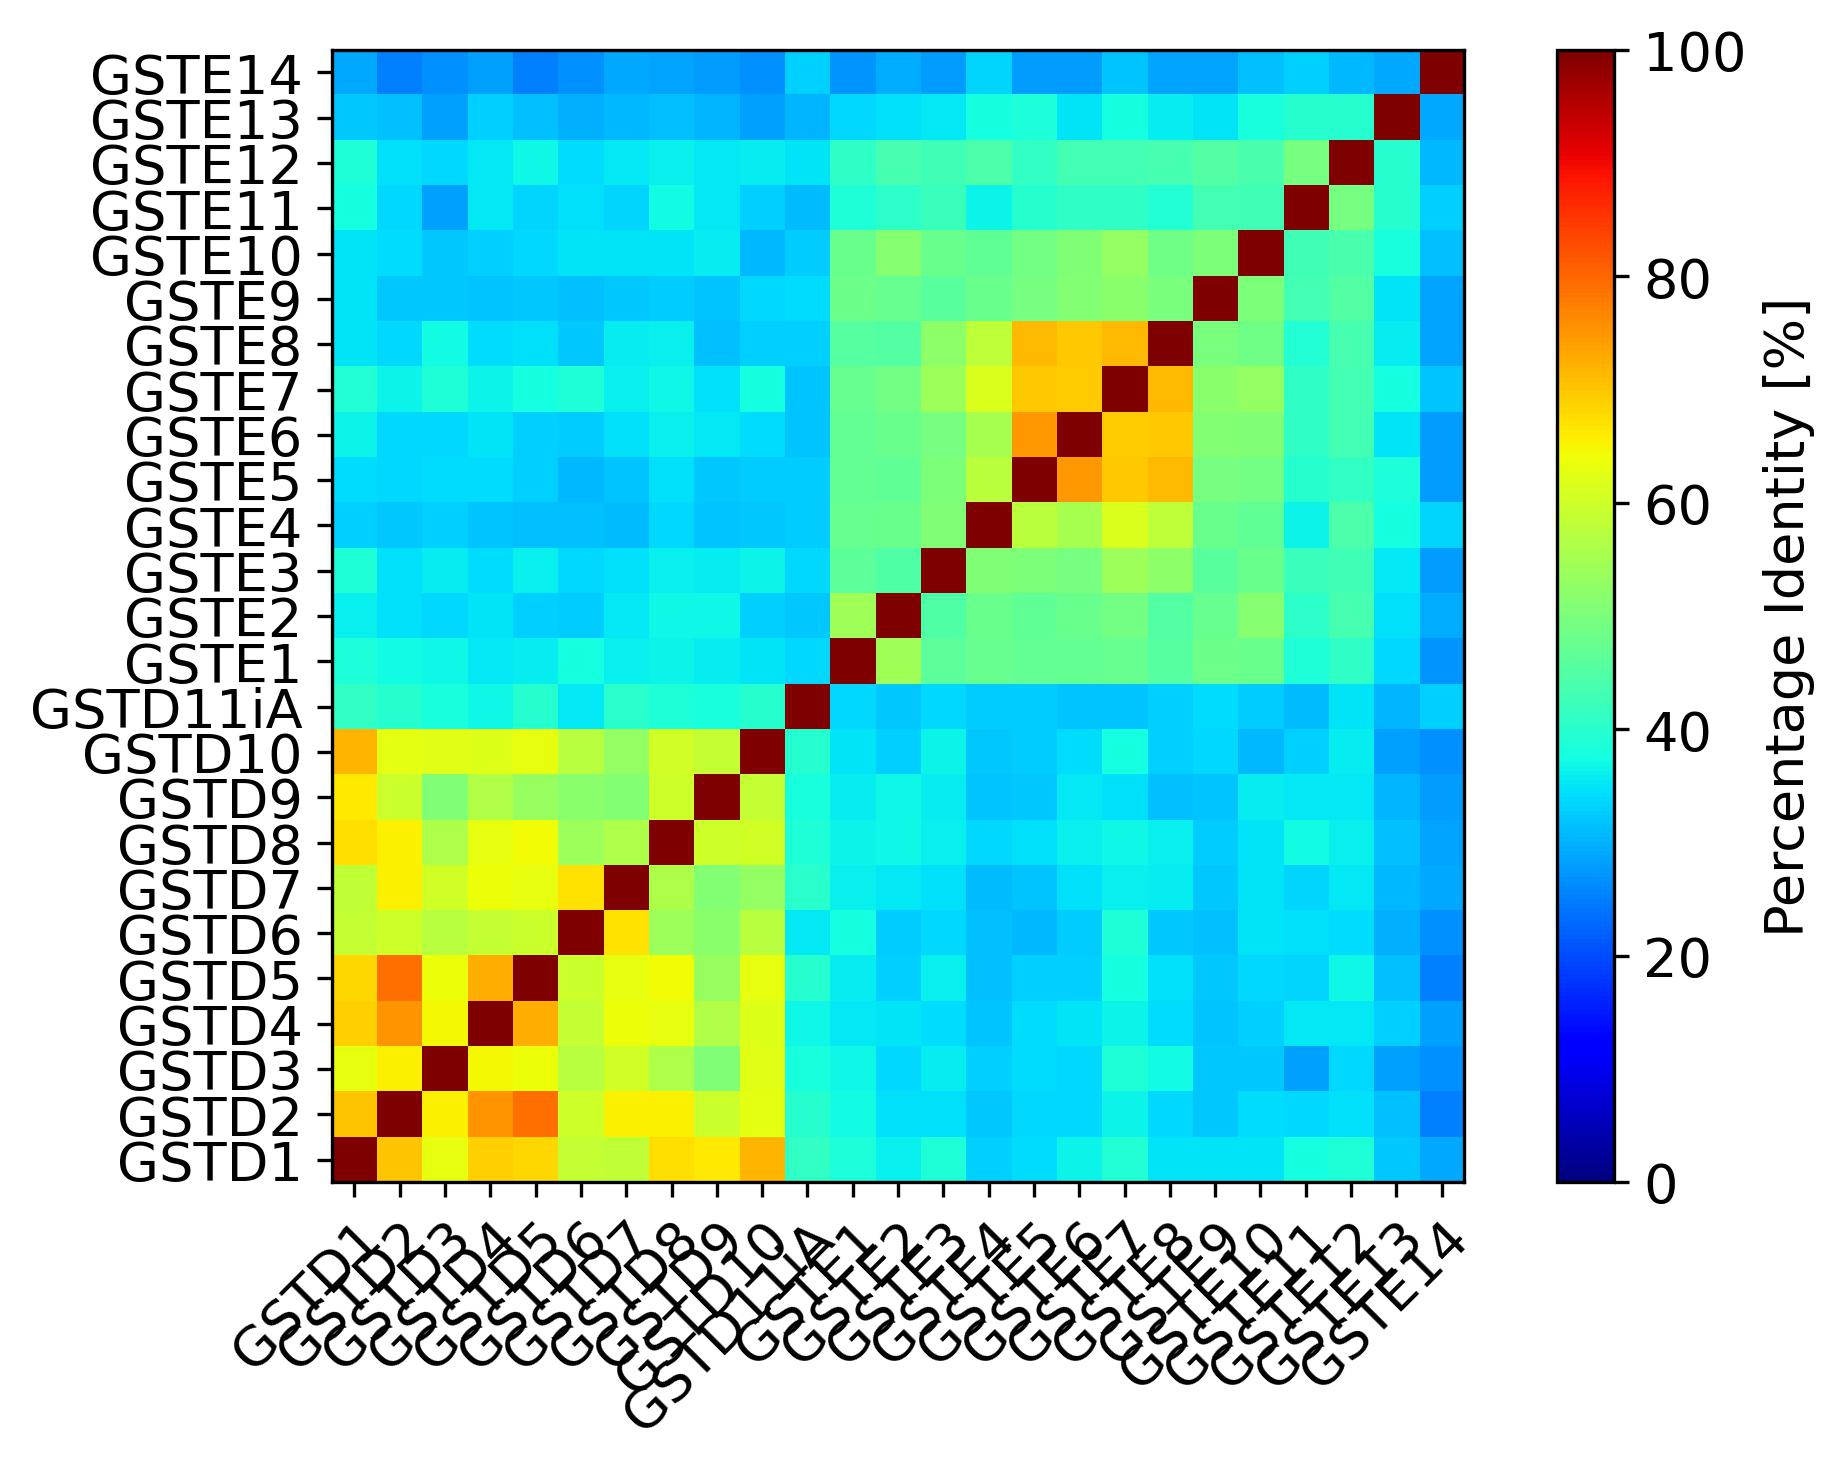
\includegraphics[width = .99\textwidth]{figures/PercentID_matrix}
	\end{minipage}
	\begin{minipage}{.32\linewidth}
		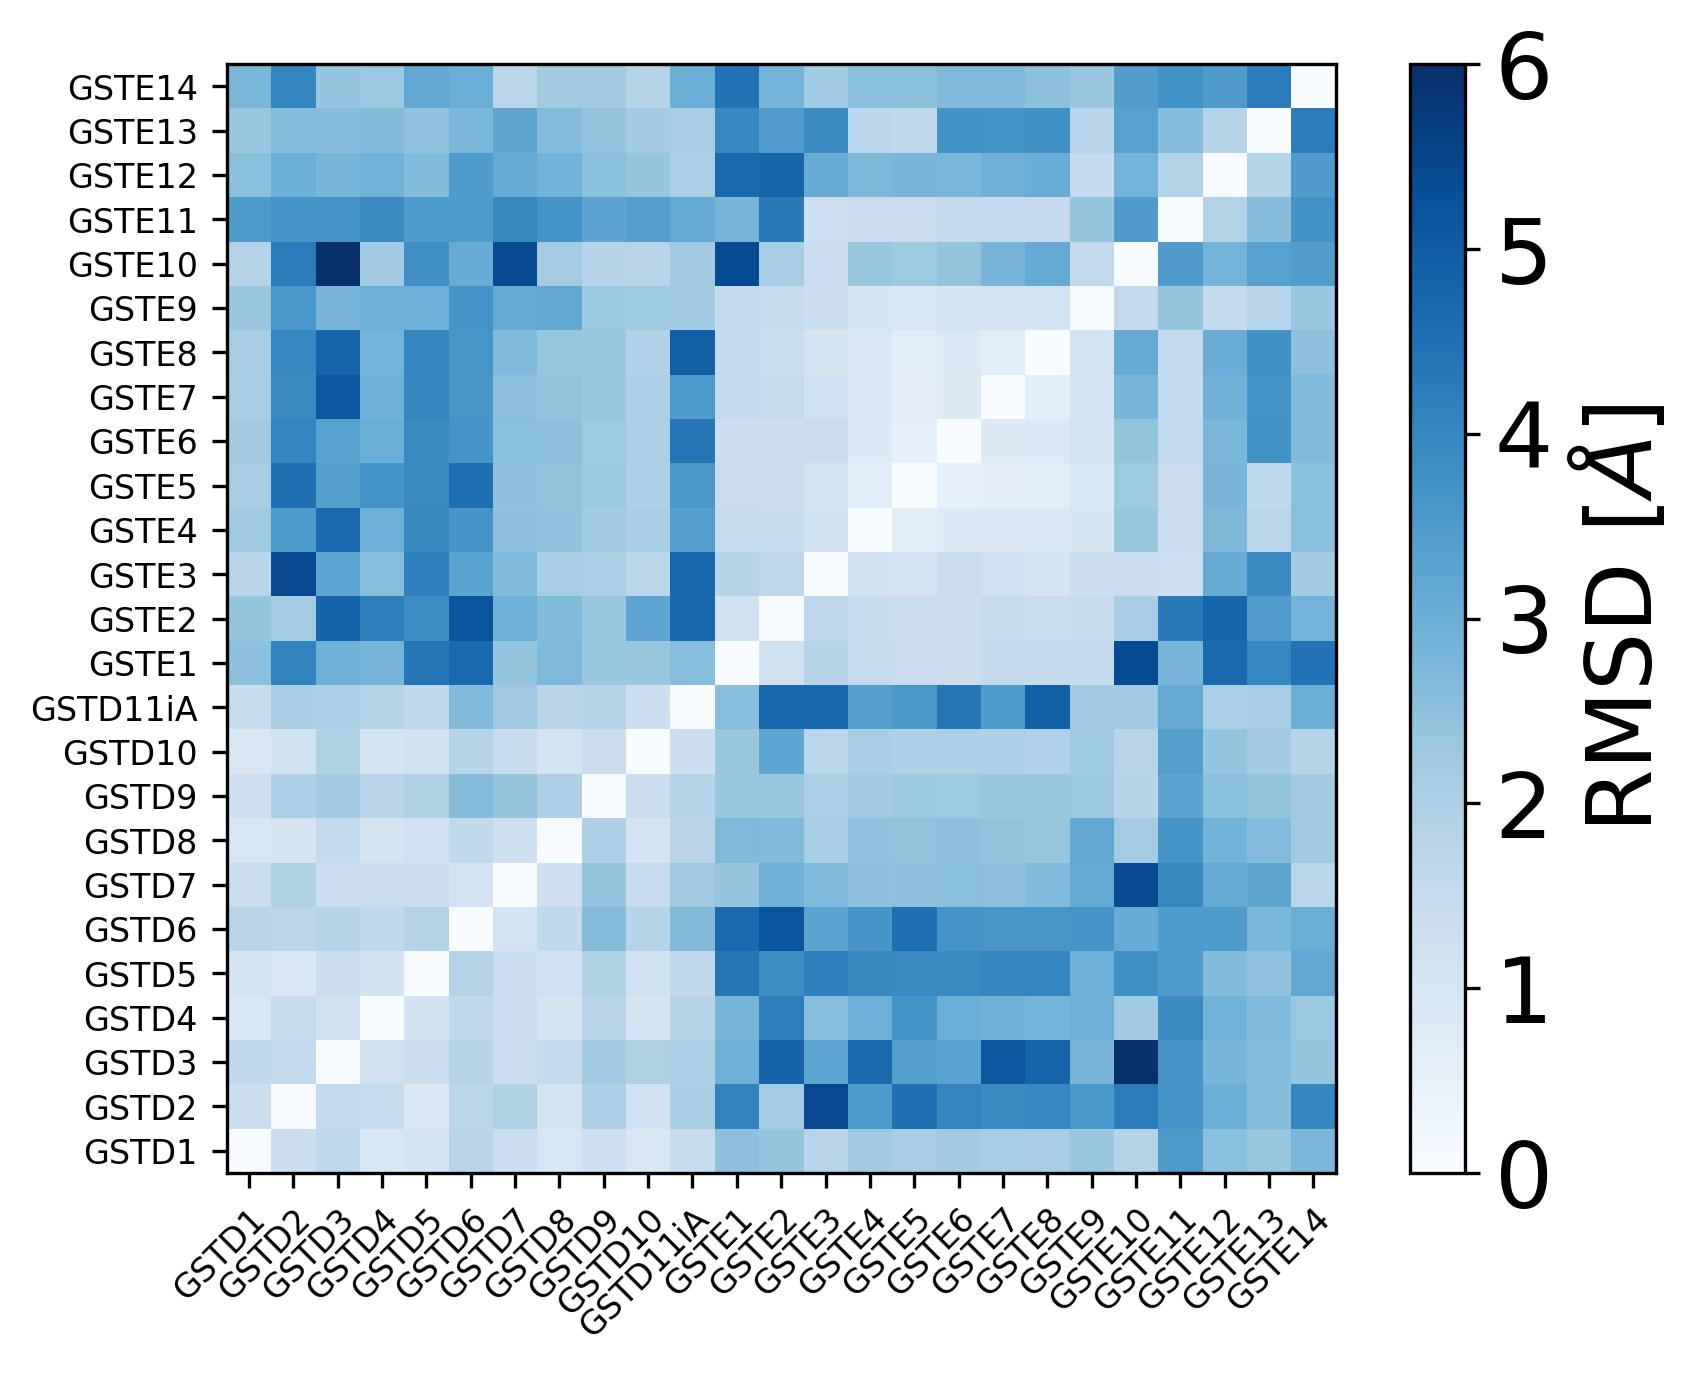
\includegraphics[width = .99\textwidth]{figures/RMSD_matrix}
	\end{minipage}
	\begin{minipage}{.32\linewidth}
		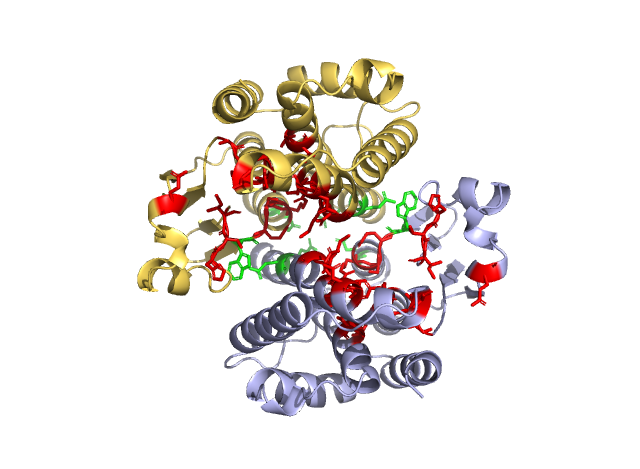
\includegraphics[width = .99\textwidth]{figures/GSTD1_DI+BS}
	\end{minipage}
	\caption{MSA \& RMSD matrix of the considered GSTs}
\end{figure}
\noindent As a preliminary analysis, the $25$ sequences of GSTs were aligned using MSA algorithms and structures were predicted using AlphaFold. The percent identity matrix has been computed and allow to show similarity between GSTs from a sequencial point of view. The proteins from class $\delta$ are all considered as part of the same cluster but for the $\epsilon$ class, some variations pears and it seems that the class itself is very heterogene. MSA also  allowed us to determine the conseved regions for the binding site (highlighted in green) and the structural differences between each structure based on the RMSD matrix. In the class $\delta$, the residues in a MSA index of $70-76$ present a very high degree of conservation, and the same goes for the residues $204-210$ in the class $\varepsilon$. Conserved regions are a first probe for the common function of proteins, mainly catalyse in the case of GSTs. Moreover, the programm AlphaFill also allows to predict the position of ligands in the structures and thuss determine the residues involved in the protein/ligands binding. Here, it clearly appears that the ligands usually binds in the regions $55-58$; $71-73$; $111-121$ with a high conservation but also in region $144-153$ of class $\varepsilon$ with a much smaller conservation. From a geometrical point of view, the structures in class $\delta$ are self similar (with RMSDs between $1$ and $2$ \AA) and structures in class $\varepsilon$ are also self similar but with some exceptions like the GSTE10, GSTE13 and GSTE14 that can either be exceptions from a biological point of view or different because of the precision of the predictions of AlphaFold (with RMSDs $\approx 4$ \AA). Finally, the interface of dimerization looks well conserved from a positional point of view but also from a chemical point of view, with a lot of chemically similar residues in the associated interfaces.   
\section{Dynamics from Normal Modes}
\begin{figure}[h!]
	\label{ANM-COM Rc param}
	\begin{minipage}{.48\linewidth}
		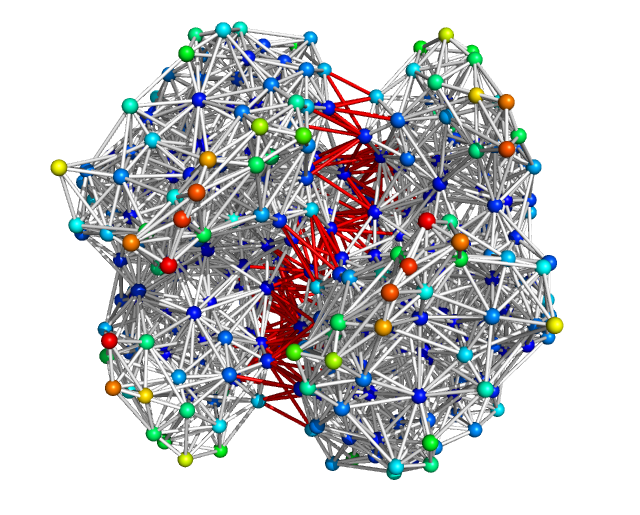
\includegraphics[width = .99\textwidth]{figures/GSTD1_ElasticNetwork.png}		
	\end{minipage}
	\begin{minipage}{.48\linewidth}
		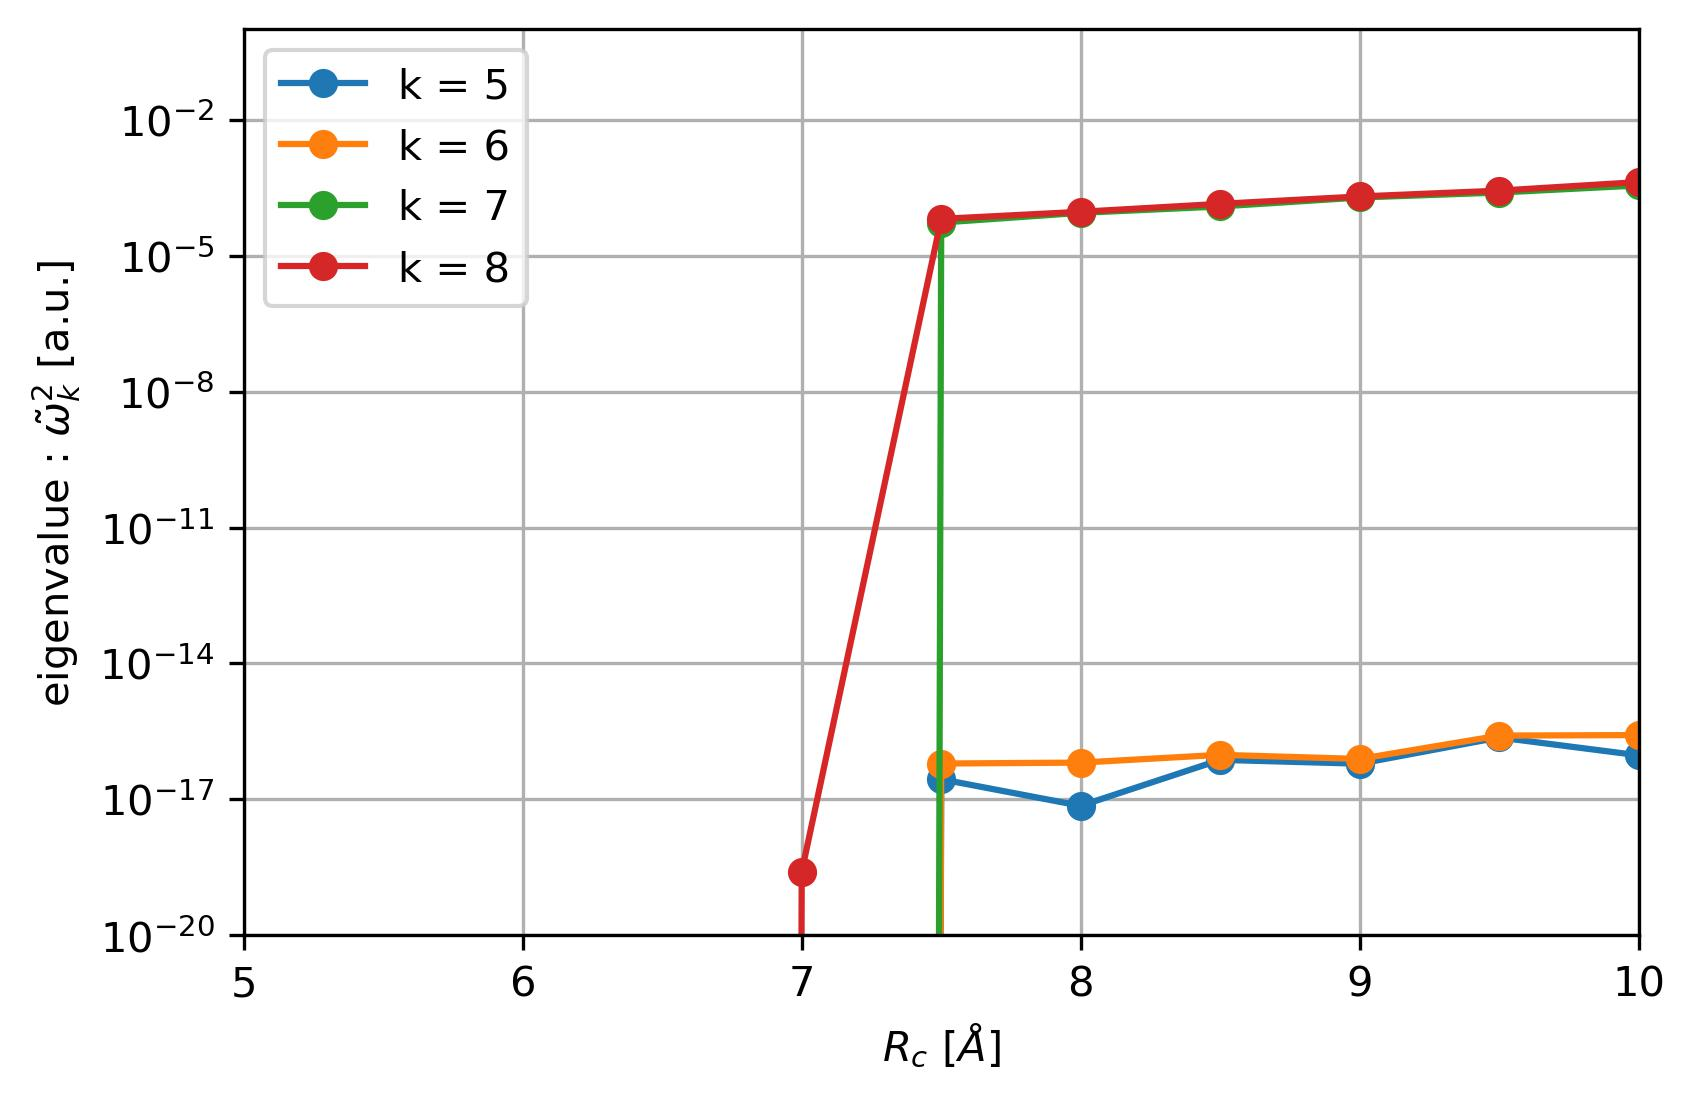
\includegraphics[width = .99\textwidth]{figures/GSTD1_ANM-COM_Rc_param}
	\end{minipage}
	\caption{ANM-COM, cut-off parametrization}
\end{figure}
\noindent As presented before, this work aim at looking at the flexibility of the structures from ANM. A very first step is to decide of a set of parameters for the model. Let us first consider the GST-D1 structure predicted from AlphaFold. As seen in equation (\ref{mass-weighted hessian matrix}), the parameter $R_c$ have a direct influence on the elements of the mass-weighted hessian $\hat{H}$ and thuss a direct influence on it's eigenvalues. The figure \ref{ANM-COM Rc param} gives a visual representation of the set of center of mass and gives the influence of $R_c$. Here, it clearly appears that the modes $5$ and $6$ are numerically nulls but the $7^{\text{th}}$ mode gets non-null for cut-off above $7.5$\AA . This specific value then is the optimal value used for the computation of collective modes (\ref{eigen equation}). 

\begin{figure}[h!]
	\label{ANM-COM Bfactors pred}
	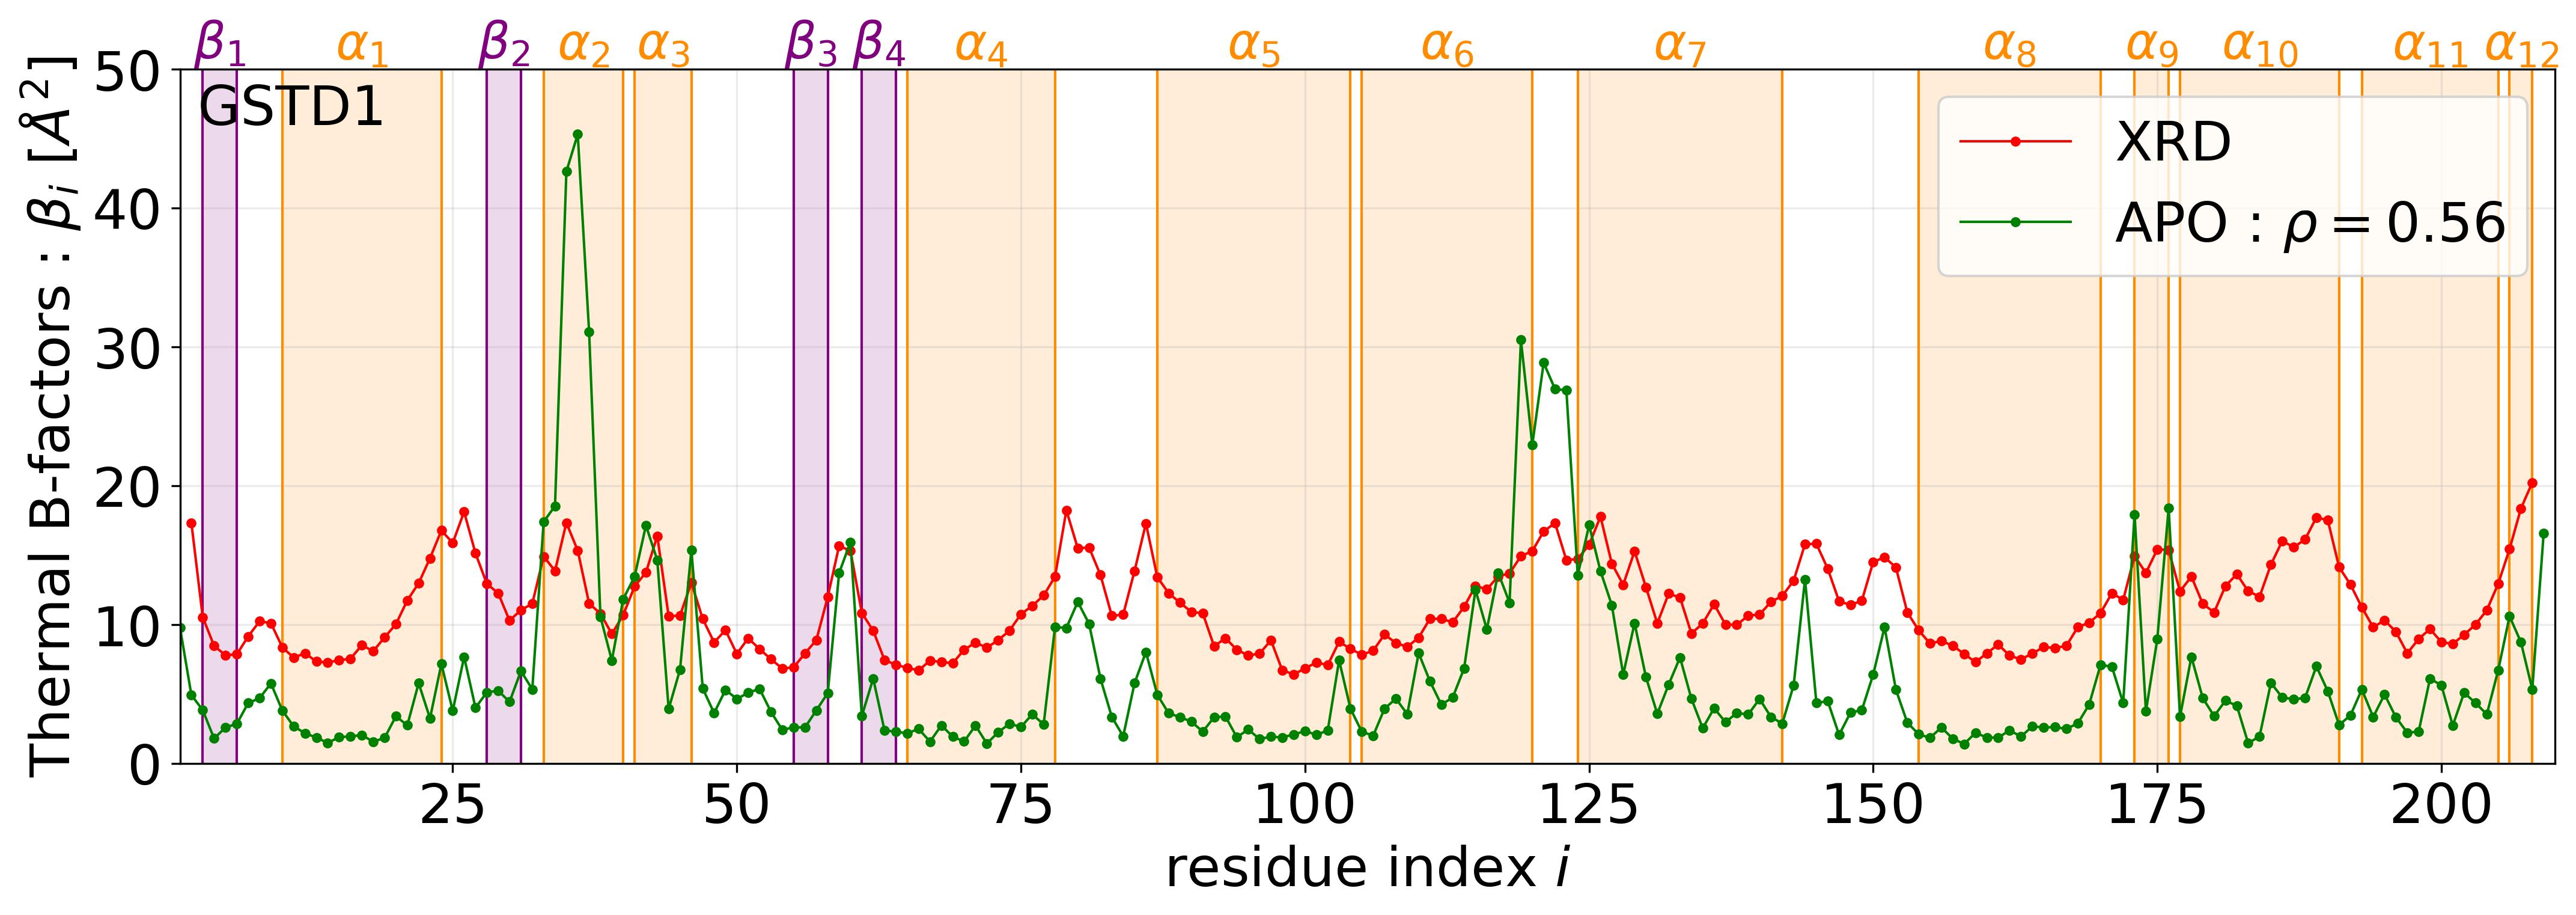
\includegraphics[width = .99\linewidth]{figures/GSTD1_ANM-COM_Bfactors.jpg}
	\caption{Thermal B-factors predictions for the AlphaFold's structure of GST-D1 and comparition with XRD experiment}
\end{figure}

\noindent From the expression (\ref{thermal B-factors}), one can plot the predicted B-factors (green curve) as well as the results from X-ray diffraction (red curve). The coefficient $\gamma$ used here is obtained using the least squared methods and gives a spring constant of $14$ kcal.mol$^{-1}$.\AA$^{-2}$. The actual precision of the measurment have been quantified based on the pearson correlation between the two series (\ref{pearsonr}) and gives $56\%$ which is a value that one can consider as descent !
\section{Dynamics from Molecular Dynamics}

\section{Comparison between Structures}